% !TEX TS-program = lualatex
% !TEX encoding = UTF-8 Unicode

\documentclass[12pt, letterpaper]{article}

%%BIBLIOGRAPHY- This uses biber/biblatex to generate bibliographies according to the
%%Unified Style Sheet for Linguistics
\usepackage[main=american, german]{babel}% Recommended
\usepackage{csquotes}% Recommended
\usepackage[backend=biber,
        style=unified,
        maxcitenames=3,
        maxbibnames=99,
        natbib,
        url=false]{biblatex}
\addbibresource{homework.bib}
\setcounter{biburlnumpenalty}{100}  % allow URL breaks at numbers
% \setcounter{biburlucpenalty}{100}   % allow URL breaks at uppercase letters
% \setcounter{biburllcpenalty}{100}   % allow URL breaks at lowercase letters

%%TYPOLOGY
\usepackage[svgnames]{xcolor} % Specify colors by their 'svgnames', for a full list of all colors available see here: http://www.latextemplates.com/svgnames-colors
\usepackage[hmargin=1in,vmargin=1in]{geometry}  %Margins          
\usepackage{graphicx}	%Inserting graphics, pictures, images 		
\usepackage{stackengine} %Package to allow text above or below other text, Also helpful for HG weights 
\usepackage{fontspec} %Selection of fonts must be ran in XeLaTeX or LuaLateX
\usepackage{amssymb} %Math symbols
\usepackage{amsmath} % Mathematical enhancements for LaTeX
\usepackage{setspace} %Linespacing
\usepackage{multicol} %Multicolumn text
\usepackage{enumitem} %Allows for continuous numbering of lists over examples, etc.
\usepackage{multirow} %Useful for combining cells in tablesbrew 
\usepackage{hanging}
\usepackage{fancyhdr} %Allows for the 
\pagestyle{fancy}
\fancyhead[L]{\textit{LING 450/550: Homework 4}}
\fancyhead[R]{Autumn 2025} 
\fancyfoot[L]{[Updated: \textit{\today}]}
\fancyfoot[C]{}
\fancyfoot[R]{\thepage} 
\renewcommand{\headrulewidth}{0.4pt}
\setlength{\headheight}{14.5pt} % ...at least 14.49998pt
% \usepackage{fourier} % This allows for the use of certain wingdings like bombs, frowns, etc.
% \usepackage{fourier-orns} %More useful symbols like bombs and jolly-roger, mostly for OT
\usepackage[colorlinks,allcolors={black},urlcolor={blue}]{hyperref} %allows for hyperlinks and pdf bookmarks
% \usepackage{url} %allows for urls
% \def\UrlBreaks{\do\/\do-} %allows for urls to be broken up
\usepackage[normalem]{ulem} %strike out text. Handy for syntax
\usepackage{tcolorbox}
\usepackage{datetime2}
\usepackage{longtable}
\usepackage{booktabs}
\usepackage{tabularx}

%%FONTS
\setmainfont{Libertinus Serif}
\setsansfont{Libertinus Sans}
\setmonofont[Scale=MatchLowercase]{Libertinus Mono}

%%PACKAGES FOR LINGUISTICS
\usepackage[noipa]{OTtablx} % Use this one generating tableaux without using TIPA
\usepackage{langsci-gb4e} % Language Science Press' modification of gb4e
\usepackage{tikz} % Drawing Hasse diagrams
\usepackage{leipzig} %	Offers support for Leipzig Glossing Rules

%%LEIPZIG GLOSSING FOR ZAPOTEC
\newleipzig{el}{el}{elder} % Elder pronouns
\newleipzig{hu}{hu}{human} % Human pronouns
\newleipzig{an}{an}{animate} % Animate pronouns
\newleipzig{in}{in}{inanimate} % Inanimate pronouns
\newleipzig{pot}{pot}{potential} % Potential Aspect
\newleipzig{cont}{cont}{continuative} % Continuative Aspect
\newleipzig{stat}{stat}{stative} % Stative Aspect
\newleipzig{and}{and}{andative} % Andative Aspect
\newleipzig{ven}{ven}{venative} % Venative Aspect
% \newleipzig{res}{res}{restitutive} % Restitutive Aspect
\newleipzig{rep}{rep}{repetitive} % Repetitive Aspect

%%TITLE INFORMATION
% \title{TITLE}
% \author{Mykel Loren Brinkerhoff}
% \date{\today}

%%MACROS
\newcommand{\sub}[1]{\textsubscript{#1}}
\newcommand{\supr}[1]{\textsuperscript{#1}}

\makeatletter
\renewcommand{\paragraph}{%
  \@startsection{paragraph}{4}%
  {\z@}{0ex \@plus 1ex \@minus .2ex}{-1em}%
  {\normalfont\normalsize\bfseries}%
}
\makeatother
\parindent=10pt


\begin{document}

%%If using linguex, need the following commands to get correct LSA style spacing
%% these have to be after  \begin{document}
    % \setlength{\Extopsep}{6pt}
    % \setlength{\Exlabelsep}{9pt}		%effect of 0.4in indent from left text edge
%%

%% Line spacing setting. Comment out the line spacing you do not need. Comment out all if you want single spacing.
%	\doublespacing
%	\onehalfspacing

\begin{center}
    {\Large \textbf{LING 450/550: Homework 4}}\\
    {\large Due: Tuesday, October 21, 2025 at 8:30am}
\end{center}
%\maketitle
%\maketitleinst
\thispagestyle{fancy}

% \tableofcontents

%------------------------------------
%\section{} \label{}
%------------------------------------

\textbf{Please read all instructions carefully before starting the assignment.} The instructions include important information for this homework. If you have any questions, please ask them in class or via email.

\begin{tcolorbox}[colback=LightGray!10!white,colframe=LightGray!75!black,title=Instructions]
    \begin{itemize}
        \item \textbf{Assignments must be written in a separate document. You cannot write on this PDF.} 
        \item Please submit your homework as a PDF file on Canvas by the deadline.
        \item You may work with other students in the class, but you must write up your solutions independently and in your own words. Please list any collaborators at the end of your assignment.
        \item You may use any resources you like, but please cite them appropriately using the \href{https://apastyle.apa.org/}{\textit{APA citation style}} or the \href{https://langsci-press.org/unifiedstylesheet}{Unified Style Sheet for Linguistics}. If you use online resources, please make sure they are reputable and reliable.
        \item Please make sure your solutions are clear and well-organized. Use headings, bullet points, and diagrams where appropriate to help illustrate your points.
        \item If you have any questions or need clarification on any part of the assignment, please don't hesitate to reach out to me or the TA via email or during office hours.
        \item \textbf{AI tools (e.g., ChatGPT, Grammarly, Copilot, etc.) can only be used to help with grammar, spelling, and formatting on this assignment. Any other use will be considered a violation of course policy and will result in a 0.}
    \end{itemize}
\end{tcolorbox}

%------------------------------------
\section*{Part 1: Vowel acoustics} \label{sec:acoustics}
%------------------------------------

Below are figures that Grant McGuire (UCSC) made from productions of monosyllabic words containing /i/, /a/, /u/ made by 60 adult speakers of American English, 30 self-identified as women, and 30 as men. He measured, using the middle 50\% of the vowel, the formants F1, F2, and F3, as well as the fundamental (f0). He also used F3 to calculate vocal tract lengths as higher formants are not available in this data set.

The figures below show F1 values by F2 values separated by gender. The data on the left panel shows the average values for each speaker. That is, each symbol represents the average F1 and F2 for a single speaker's vowel production. The right figure shows the average value for each gender, so the yellow <i> symbol represents the F1 and F2 values for all the women’s productions of /i/.

\begin{center}
    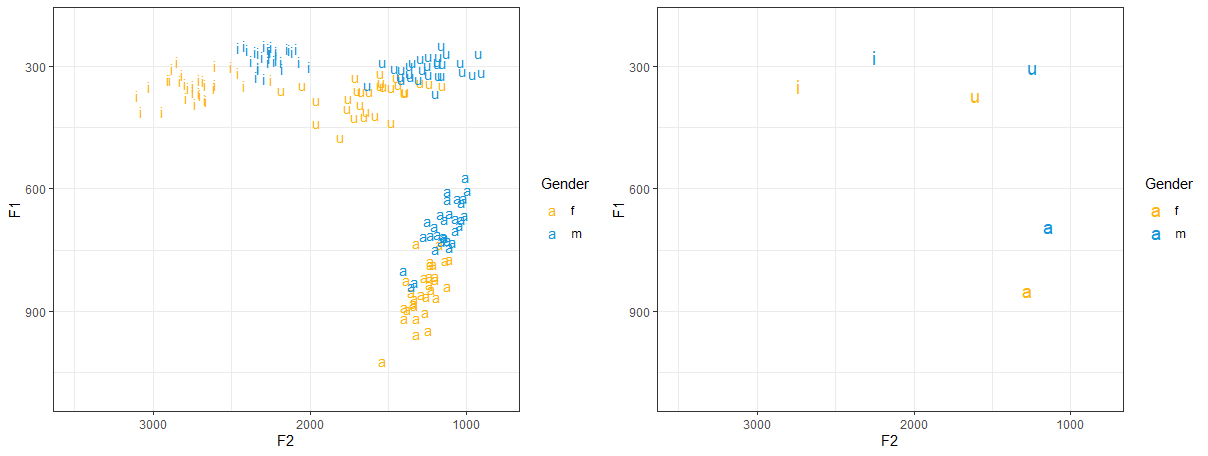
\includegraphics[width = \textwidth]{figs/vowel_data.jpg}
\end{center}

The figures below are similar, but show the fundamental frequency, f0, plotted against the vocal tract length (in cm). As above, the left panel has averaged values for each speaker and vowel, and the right panel shows it averaged by gender and vowel.

\begin{center}
    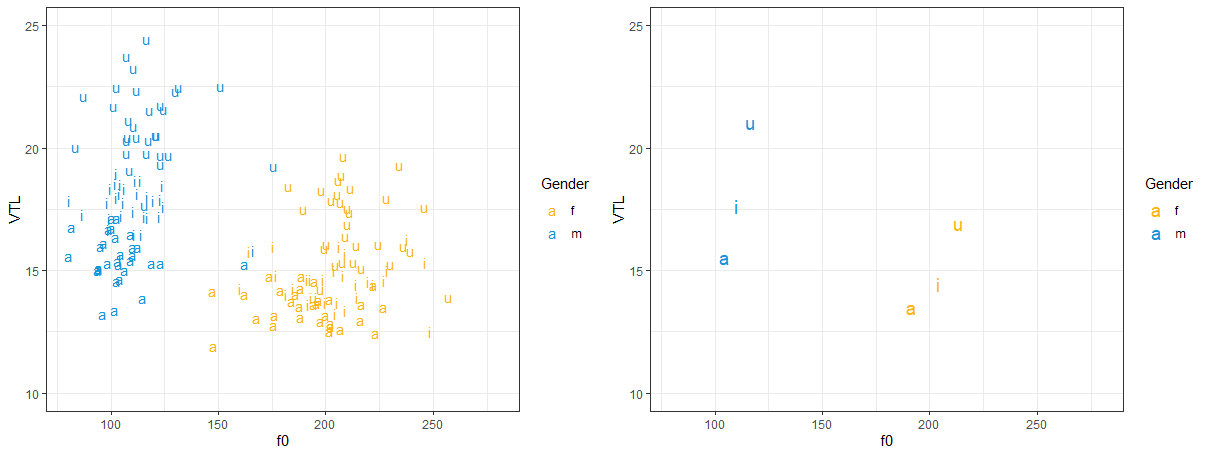
\includegraphics[width = \textwidth]{figs/vtl.png}
\end{center}

Answer the following questions about these data (Be as clear and specific as possible, each answer should be a paragraph, at least.)

\begin{enumerate}
    \item The men’s and women’s formant values are systematically different. What accounts for this?
    \item The men’s and women’s fundamentals are systematically different. What accounts for the difference?
    \item The longest vocal tract is derived from /u/. Can you give two reasons why? Use the perturbation theory for one explanation, and refer to tube models for the other.
\end{enumerate}


%------------------------------------
\section*{Part 2: Your vocal tract length} \label{sec:spectra}
%------------------------------------

Calculate the length of your vocal tract, in centimeters, by recording the example words given below. Use F1, F2, F3, and F4 calculated from productions of /i/, /a/, /u/, /æ/, and /ə/, as well as a mean value, for example: F1\textsubscript{mean} = (F1\textsubscript{i} +F1\textsubscript{a} +F1\textsubscript{u} +F1\textsubscript{æ} +F1\textsubscript{ə} )/5. Which calculation is the least variable, and therefore most reliable? How do you know? Please report all values in a table like the one below. How do they compare to the lengths calculated in the data for Part 1?

\begin{table}[h!]
\renewcommand{\arraystretch}{1.3}
\caption{Formant frequencies for selected vowels}
\centering
\begin{tabularx}{\textwidth}{|c|X|X|X|X|X|X|}
\hline
 & \textit{fleece} [i] & \textit{lot} [a] & \textit{goose} [u] & \textit{trap} [æ] & \textit{about}$^{3}$ [ə] & Mean of all vowels \\
\hline
F1 &  &  &  &  &  &  \\
\hline
F2 &  &  &  &  &  &  \\
\hline
F3 &  &  &  &  &  &  \\
\hline
F4 &  &  &  &  &  &  \\
\hline
\end{tabularx}
\end{table}

\textit{Hints to help solve this.}
Finding formants in Praat is easy
\begin{itemize}
    \item Put the cursor in the middle of the vowel you are measuring.
    \item Press the function key (\texttt{Fn}) corresponding to the formant, so \texttt{Fn1} = gives you the first formant, \texttt{Fn2} = second formant, etc.
    \item \textbf{Be careful, Praat doesn’t always track formants well}, so you may need to check by hand, either making a spectrum (highlight a section, \texttt{CTRL-L} or \texttt{CMD-L}) or put the cursor in the middle of the formant and check the frequency it reports on the left of the display.
\end{itemize}

Formula for calculating the vocal tract length from a formant frequency:
\begin{equation*}
    L = \frac{(2n-1)c}{4f}
\end{equation*}
\begin{itemize}
    \item $n$ = the formant number you are measuring, e.g. n = 1 for F1, n = 2 for F2, etc.
    \item $c$ = 350m/s, or 35000cm/s
    \item $f$ = the frequency, in Hz, of the formant in question.
    \item an excel version of this formula would look something like:
    \begin{itemize}
        \item 
        \begin{verbatim}
            ((2*cell1-1)*35000)/(4*cell2)
        \end{verbatim}
        \item Where cell1 = the n cell address, and cell2 = the formant frequency cell address
    \end{itemize}
    \item Be careful of your units!
    \item Human vocal tracts are usually somewhere between 12cm and 22cm, anything much larger or smaller than this suggests a problem in your calculations.
\end{itemize}

%------------------------------------
%BIBLIOGRAPHY
%------------------------------------

%\singlespacing
%\nocite{*}
% \printbibliography[heading=bibintoc]

\end{document}